\documentclass[11pt,a4paper]{article}
\usepackage{fontspec}
\usepackage{amsmath}
\usepackage{amsfonts}
\usepackage{amssymb}
\usepackage{graphicx}
\usepackage{hyperref}
\usepackage{dirtytalk}
\usepackage{caption}
\usepackage{subcaption}
\usepackage{listings}
\usepackage{tikz}
\usepackage{import}
\usepackage[perpage]{footmisc}
\usepackage[margin=2.5cm]{geometry}
\usepackage[subpreambles=true]{standalone}

\setlength\parindent{0pt}
\captionsetup{format=hang}
\setcounter{MaxMatrixCols}{20}


\author{Leonard Bruns $<$\href{mailto:leonardb@kth.se} {leonardb@kth.se}$>$}
\title{OST-HMD Calibration}


%\renewcommand{\refname}{Relevant Papers}

\begin{document}
	\maketitle
	\tableofcontents
	\section{Basic concepts}
	\emph{Odometry} in general refers to the process of inferring the movement of a mobile robot by the use of motion sensors. An example would be the use of the encoders measuring the rotation of wheels. Given the geometry of the wheels the velocity can be inferred and integrating this will result in a path.
	
	The problem with odometry is that errors in the measurement or due to unmodelled factors (like slippage on the ground or inside the transmission) can not be accounted for by the odometry alone and thus the error grows due to the integration over time.
	
	As explained before odometry suffers from drift, which can not be accounted for. Also, even if there would be no drift or it would be so small that it does not matter for a given application, it would only allow the robot to position itself relative to its starting point. Thus without any extra information like a starting point relative to a map it is not possible to position the robot.
	
	\emph{Dead reckoning} describes the process of inferring the position by using and integrating kinematic values (i.e. position, velocity, acceleration, orientation, radial velocity, radial acceleration). It is closely related to odometry in that odometry uses dead reckoning to infer the position.
	
	The \emph{extended Kalman filter} or \emph{EKF} is based on linearizing not linear motion models. While this approach works well if a given state is close to the real state it becomes tricky if the estimated state is of, which might cause the algorithm to not converge to the correct position. Especially if the initial state is unknown this can prove to be problematic.
	
	\emph{SLAM (simultaneous localization and mapping)} describes the problem of positioning a robot inside an unknown environment by doing both, localizing it inside this environment and building a map of the environment. 
	
	\emph{Occupancy grids} is a gridded approach to map building and description. The map is devided into grids and each grids can be either occupied or non-occupied, meaning there is or is no obstacle at this specific grid position.
	
	\emph{Particle filters} are an alternative way to deal with nonlinear motion and measurement models. Instead of linearizing the equation it samples from the nonlinear distributions and thus always approximates the non gaussian probability distribution. Due to its nature it is quite easy to implement (no linearization required) and allows for much more complex measurement and motion models. On the otherhand it is computationally expensive since a large number of samples is required to make the algorithm robust. In addition it will always be a probabilistic approach and unlucky samples might cause the algorithm to give bad estimates. Also is all samples are once stuck in an unlikley area the basic algorithm will not automatically detect such a situtation as it keeps resampling from the current distribution. Thus it might take a long time or it might never recover the correct position. There are however different adjustments to the algorithm which deal with these shortcomings.
	
	The main challenges in robotics navigation is to build a system robust enough to deal with a dynamically changing environment. Understanding what are outliers and what are actual obstacles seems  to be very difficult.
	
	A \emph{holonomic} robot is a robot that can move directly in every direction (holonomic is only defined in relation to certain number of dimensions). An example for a non-holonomic robot would be a car, as that can only move forward and backwards, not directly to the left or right. 
	
	\section{Localization}
	\subsection{Theory}
	The given data is comprised of timestamped
	\begin{itemize}
	    \item GPS measurements
	    \begin{itemize}
	        \item $x,y,z$ values in $\mathrm{m}$, with $z$ being the height
	        \item $HDOP$ and $VDOP$, describing the expected quality of the measurements
	    \end{itemize}
	    \item Speedometer measurements in $\mathrm{m}/\mathrm{s}$
	    \item IMU measurements
	    \begin{itemize}
	        \item acceleration $a_\mathrm{x},a_\mathrm{y},a_\mathrm{z}$ in $\mathrm{m}/\mathrm{s}$
	        \item radial velocity $\omega_\mathrm{x}, \omega_\mathrm{y}, \omega_\mathrm{z}$, corresponding to the radial velocity around the respective axis in $\mathrm{rad}/\mathrm{s}$
	    \end{itemize}
	\end{itemize}
	After analyzing the data it was found that the IMU is apparently mounted on the vehicle such that its $x$ axis aligns with the driving direction and the $z$ axis represents the main rotational axis of the vehicle. In addition it was observed that the distance travelled according to the GPS and speedometer is about $2\mathrm{km}$ in the  xy-plane and about $80m$ ($40\mathrm{m}$ down and $40\mathrm{m}$ up) in the z-direction. Due to time constraints the problem has been simplified to a 2D problem only incorporating the xy-coordinates of the car, its orientation inside this plane and its forward velocity.
	
	An \emph{extended Kalman filter (EKF)} is suitable for such a situation. As it provides easy means of fusing the different measurements and representing the distribution of the position using a Gaussian. A Kalman filter is not suitable, since that would require a linear motion and measurement model, which is not the case as shown below. A particle filter would also work, but is computationally more expensive, and since the data should yield a unimodal distribution it does not seem to be worth it.
	
	The state of the system at timestep $k$ is thus given by
	\begin{equation}
	    \mathbf{x_k}=\begin{bmatrix}
	        x_k\\
	        y_k\\
	        \theta_k \\
	        v_k
	    \end{bmatrix}.
	\end{equation}
	The IMU measurements, which are the most frequent measurements, are taken as the control input
	\begin{equation}
	    \mathbf{u_k}=\begin{bmatrix}
	        \omega_k \\
	        a_k
	    \end{bmatrix}.
	\end{equation}
	A simple motion model using constant velocity between timesteps and constant orientation between two timesteps has been chosen. The transition function describing the motion of the robot based on the current state, the control input and the noise $v$ is then given by
	\begin{equation}
	    \mathbf{\hat{x}_k}=f(\mathbf{\hat{x}_{k-1}},\mathbf{u_k},\mathbf{w_{IMU,k}})=
	    \begin{bmatrix}
	        x_{k-1}+v_{k-1}\cos{(\theta_{k-1})}\Delta t \\
	        y_{k-1}+v_{k-1}\sin{(\theta_{k-1})}\Delta t \\
	        \theta_{k-1}+(\omega_k+w_{\omega,k})\Delta t \\
	        v_{k-1}+(a_k+w_{a,k})\Delta t
	    \end{bmatrix}.
	\end{equation}
	As stated above it can easily be seen that this is not a linear function of the previous state and control input, which is why an EKF has to be used instead of a normal Kalman filter.
	
	The noise term $\mathrm{w_{IMU,k}}$ describes the noise in the IMU measurements. Inside the prediction step of the EKF it will be set to 0, but its covariance $\mathbf{Q_{IMU}}$ is used to update (increase) the estimate's covariance during the prediction step.
	
	The measurement models of GPS and the speedometer are straightforward in that they simply measure the respective states and are thus not explained in further detail.
	
	\subsection{Implementation and Results}
	The previously discussed EKF was first implemented in Matlab to prototype it and find decent values for the covariance matrices $\mathbf{Q_\mathrm{IMU}}, \mathbf{Q_\mathrm{GPS}}$ and $\mathbf{Q_\mathrm{speedometer}}$. Results as well as results when removing some sensors can be seen in Figure \ref{fig:ekf}. After that the same filter has been implemented in C++ using the Eigen library for the matrix operations. A simple realtime visualization in RViz was implemented as well.
	
	\begin{figure}[htp]
	    \centering
	    \begin{subfigure}[b]{0.48\textwidth}
	        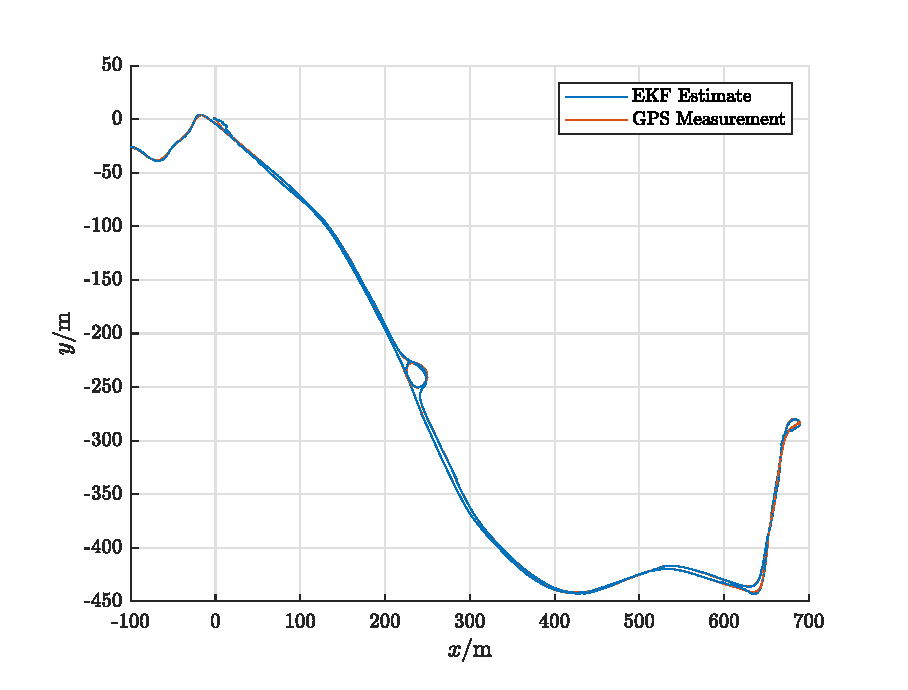
\includegraphics[width=\textwidth]{figures/ekf_estimate.eps}
	        \subcaption{EKF and GPS trajectory}
	    \end{subfigure}
	    \begin{subfigure}[b]{0.48\textwidth}
	        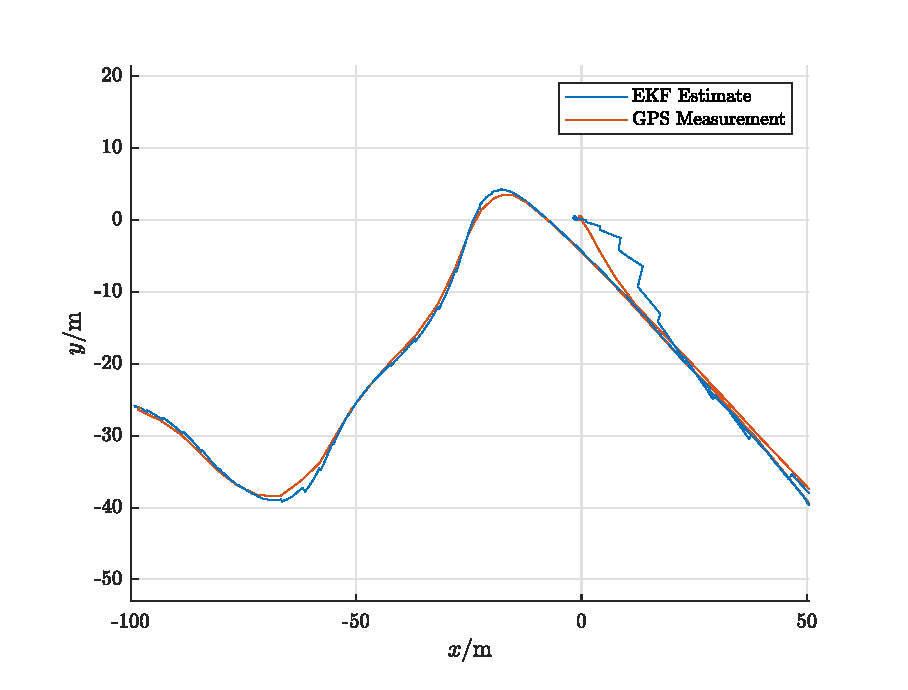
\includegraphics[width=\textwidth]{figures/ekf_estimate_zoom.eps}
	        \subcaption{Zoomed part of (a)}
	    \end{subfigure}
	    
	    \begin{subfigure}[b]{0.48\textwidth}
	        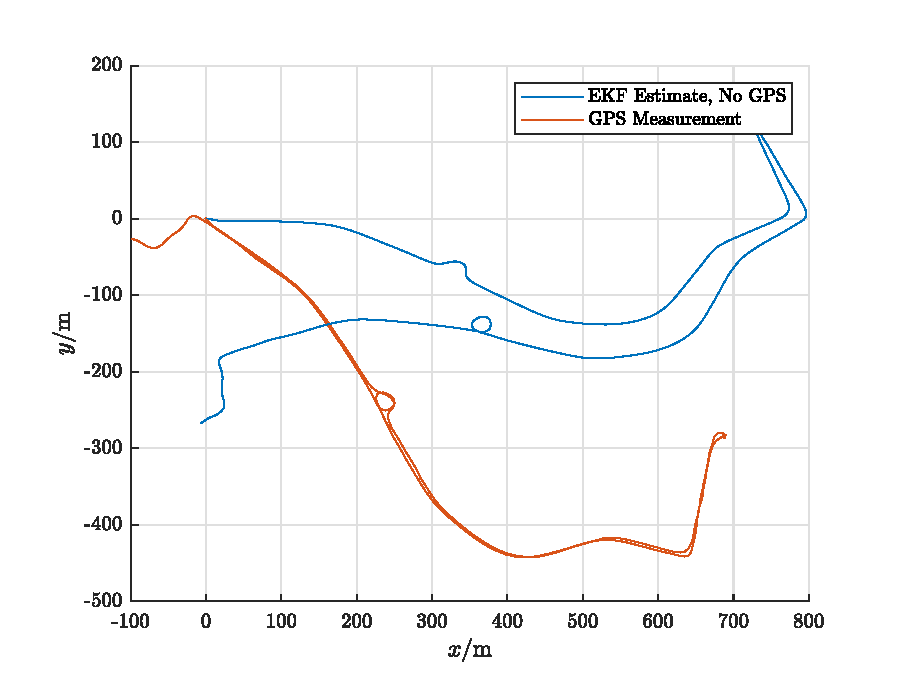
\includegraphics[width=\textwidth]{figures/no_gps.eps}
	        \subcaption{No GPS}
	    \end{subfigure}
	    \caption{(a) shows both the trajectory based on the GPS only as well as the EKF estimating the trajectory based on GPS, IMU and speedometer. (b) shows a zoomed portion of this plot. It can be seen that the filter will take some timesteps to get find the correcft orientation and to converge to the right track. When returning after taking the long path, the trajectory aligns well with the GPS trajectory. (c) shows the difference when the GPS measurement update is omitted inside the EKF. It can be seen that it is impossible for the EKF to find the same real world orientation as well as drifting away due to measurement noise. The general shape of the two trajectories is the same though.}
	    \label{fig:ekf}
	\end{figure}
	
	\subsection{Outlook and Discussion}
	The EKF was successfully implemented and in general seems to give reasonable estimates. In the beginning it can be seen that it takes some time to find the correct orientation, using the GPS measurements. The model would easily be extensible with additional sensor data and the underlying motion model could easily be changed. 
	
	Of course by discarding measurements like the acceleration in y direction information is lost, which could otherwise be used to improve the model accuracy. In this case having an easy motion model was chosen to have a good basis to built upon and to get insight into the underlying formulas.
	
	In addition it should be noted that the IMU data is not well scaled and probably biased, but due to limited information available it is not possible to calibrate for that.
	
	If one measurement is delayed the algorithm will deal with it correctly, the noise term will just grow more. If the IMU is damaged and does not give any readings the GPS measurements will cause the estimate to stay approximately at the right spot and follow the path, but more accurate estimation is hardly possible or realiable. How exactly the noise term is affected depends on whether the prediction step is still performed or not. In general the GPS measurements should be able to recover the robot's position in a kidnapped robot situation.
	\bibliographystyle{ieeetr}
	\bibliography{library}
\end{document}